We first give more details on the equivalence between \mmc{} and \pcc{},
following~\autocite{Demaine2006} but omitting the full proofs to avoid redundancy. Recall that given
a weighted graph $H=(V_H, E_H, w_H)$ and a collection of $k$ sources and targets
$S=\{(s_i,t_i)\}_{i=1}^k \in V_H^2$, in \mmc{} we want to find the lightest set of edges $T\in E_H$
whose removal disconnects every pair $s_i$ from the corresponding $t_i$. Let us first describe a
polynomial reduction from \mmc{} to \pcc{}. Namely, given an instance $(H, S)$ of \mmc{}, we let
$W_H=\sum_{e\in E_H} w_H(e)$ be the total weight of $H$ and $G_H$ be the same graph as $H$ with all
its edges labeled positively. We then connect every pair $(s_i, t_i)$ by a negative edge of weight
$W_H+1$. One can check (\autocite[Theorem 4.7]{Demaine2006}) that a multicut $T$ in $H$ with weight
$W$ induces a clustering in $G_H$ of weighted disagreement $W$ by the connected components of
$G^+\setminus T$. Likewise, a clustering of $G_H$ with weight $W$ induces a multicut on $H$ with
weight as most $W$. In the unweighted case, the reduction is similar but the heavy negative edges
are simulated in the following way: include every source and target in a clique of $n$ nodes and
connect that clique to the corresponding source or target by $n$ negative edges.

We next present the polynomial reduction from \pcc{} to \mmc{}. Given $G=(V, (E^+, E^-), w)$ we let
$H_G$ be the graph induced by $E^+$ with the same weight. Then for every negative edge $(u,v)$ of
weight $w_{uv}^-$, we create a new vertex $v_{\widehat{uv}}$, connect $u$ to $v_{\widehat{uv}}$ with
weight $w_{uv}^-$ and let $(v_{\widehat{uv}}, v)$ be a source-target pair added to $S_G$. This
construction is depicted in \autoref{fig:cc_mmc} and one can show (\autocite[Theorem
4.4]{Demaine2006})\Todo{give the intuition of the proof} that it takes a linear time to construct a
multicut of weight $W$ in $H_G$ from a clustering of weight $W$ in $G$, and vice versa.

\begin{figure}[htpb]
   \centering
   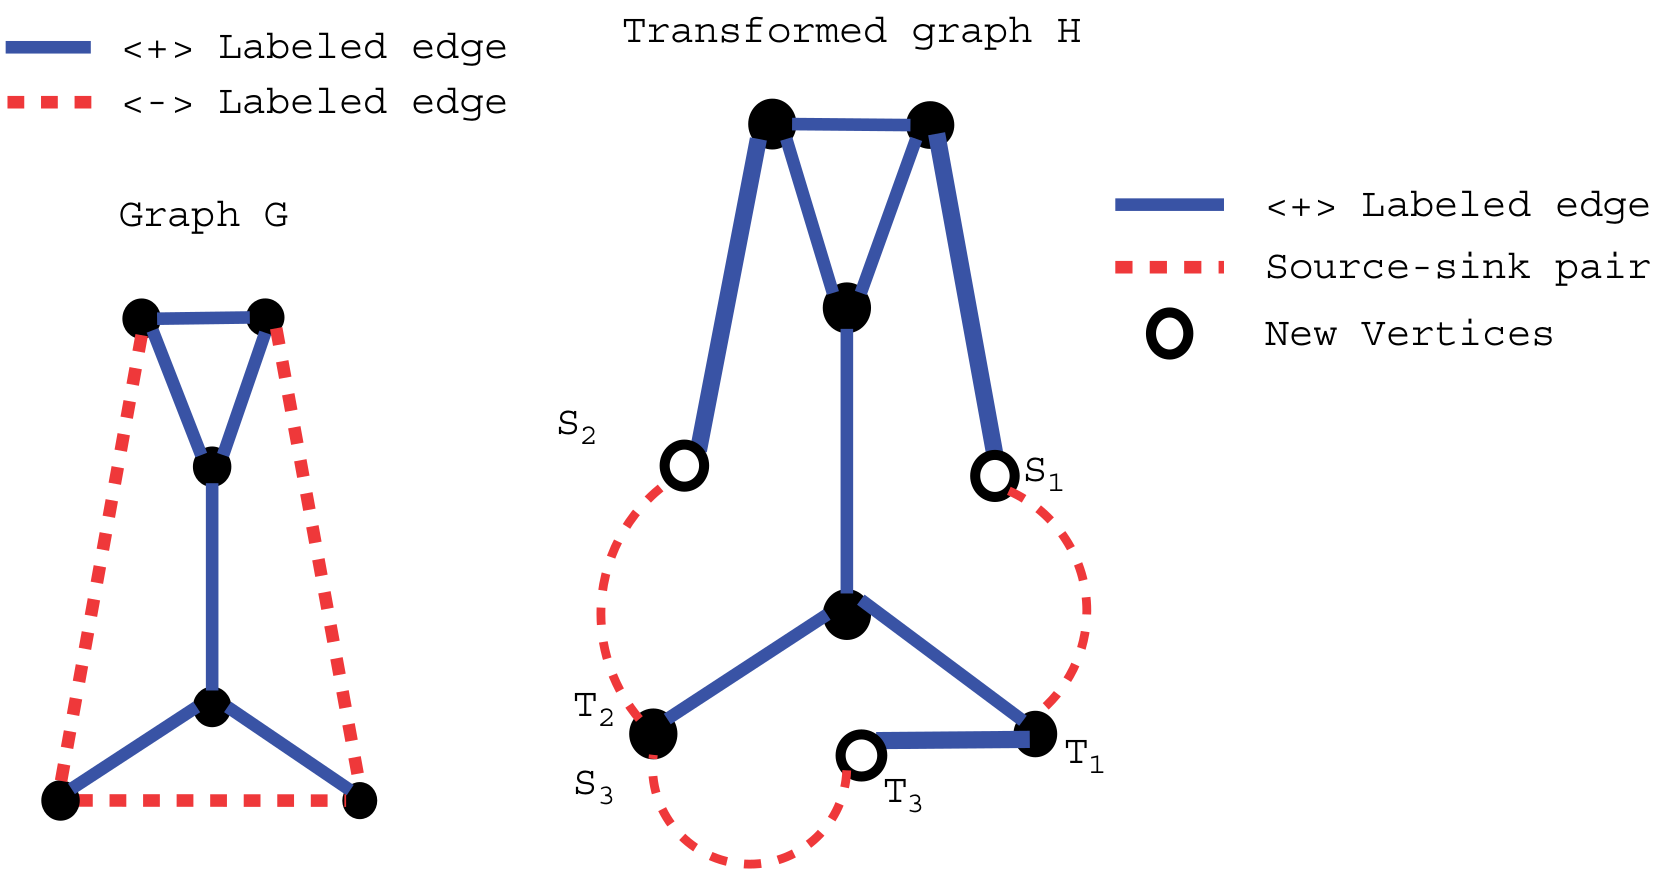
\includegraphics[width=0.8\linewidth]{assets/raw/cc_to_mmc.png}
   \caption{The transformation from \pcc{} on $G$ to \mmc{} on $H$ (temporarily reproduced from
   \autocite{Demaine2006}) \label{fig:cc_mmc}}
\end{figure}

\url{http://fpt.wikidot.com/fpt-races} and
\url{http://fpt.wikidot.com/complexity-status-of-edge-modification-problems} for parameterized
papers on \mmc{} and \textsc{Cluster Editing}.


Whereas clustering objective functions are \NPh{} to optimize, we expect that meaningful instances
in which we are interested have additional structure which allows for guaranteed polynomial time
algorithms, see for instance \autocite{clusteringFeasibility15} for a critical overview of some
proposed such notions of structure. Informally, a general idea is that the clustering should not
change (or at least very little) if the data are slightly perturbed. For instance, a weighted graph
is \emph{$\alpha$-stable} (with $\alpha>1$) for some partition objective if its optimal partition
remains the same whenever every weight $w_i$ is multiplied by a factor $c_i$ between $1$ and
$\alpha$. Finally, we say that an algorithm is \emph{robust} if, given an instance $\mathcal{I}$ and
in polynomial time, it: returns the optimal solution of $\mathcal{I}$ if $\mathcal{I}$ is
$\alpha$-stable; and if $\mathcal{I}$ is not $\alpha$-stable, either returns the optimal solution of
$\mathcal{I}$ or reports that $\mathcal{I}$ is not $\alpha$-stable. This is a handy property, as in
general, we cannot check the stability of an instance in practice as we do not know the optimal
solution hence we cannot tell whether it changes or not under perturbations.

\Textcite{StableCC17} provide a robust algorithm for $2-\nicefrac{2}{k}$-stable instance of
$k$-\textsc{Minimum Multiway Cut}, which therefore is not really useful in our case because I confused
multiway cut and multicut. To be fair, it seems I'm not the only one, \href{http://pages.cs.wisc.edu/~shuchi/papers/multicut-hardness-full.pdf}{on the hardness of
   approximating multicut}
   \enquote{multicut is known to be APX-hard
      (\href{https://pdfs.semanticscholar.org/1cf6/4c2bdd4f1c384a55910606a64c8d831a96ba.pdf}%
   {Dahlhaus et al. 1994}).} by that 1994 paper define the multiway cut problem, see
   \autoref{fig:cc_multiwhat}. \Textcite[Theorem 24]{Bansal2004} show that we can go from
   \textsc{Minimum Multiway Cut} to \pcc{} but I doubt about the other direction, mostly because
   \textsc{Minimum Multiway Cut} can actually be approximated with factor smaller than $1.3$.
   see \url{http://www.nowozin.net/sebastian/papers/nowozin2009lpstability.pdf} about LP multicut
   stability.
\begin{figure}[htpb]
   \centering
   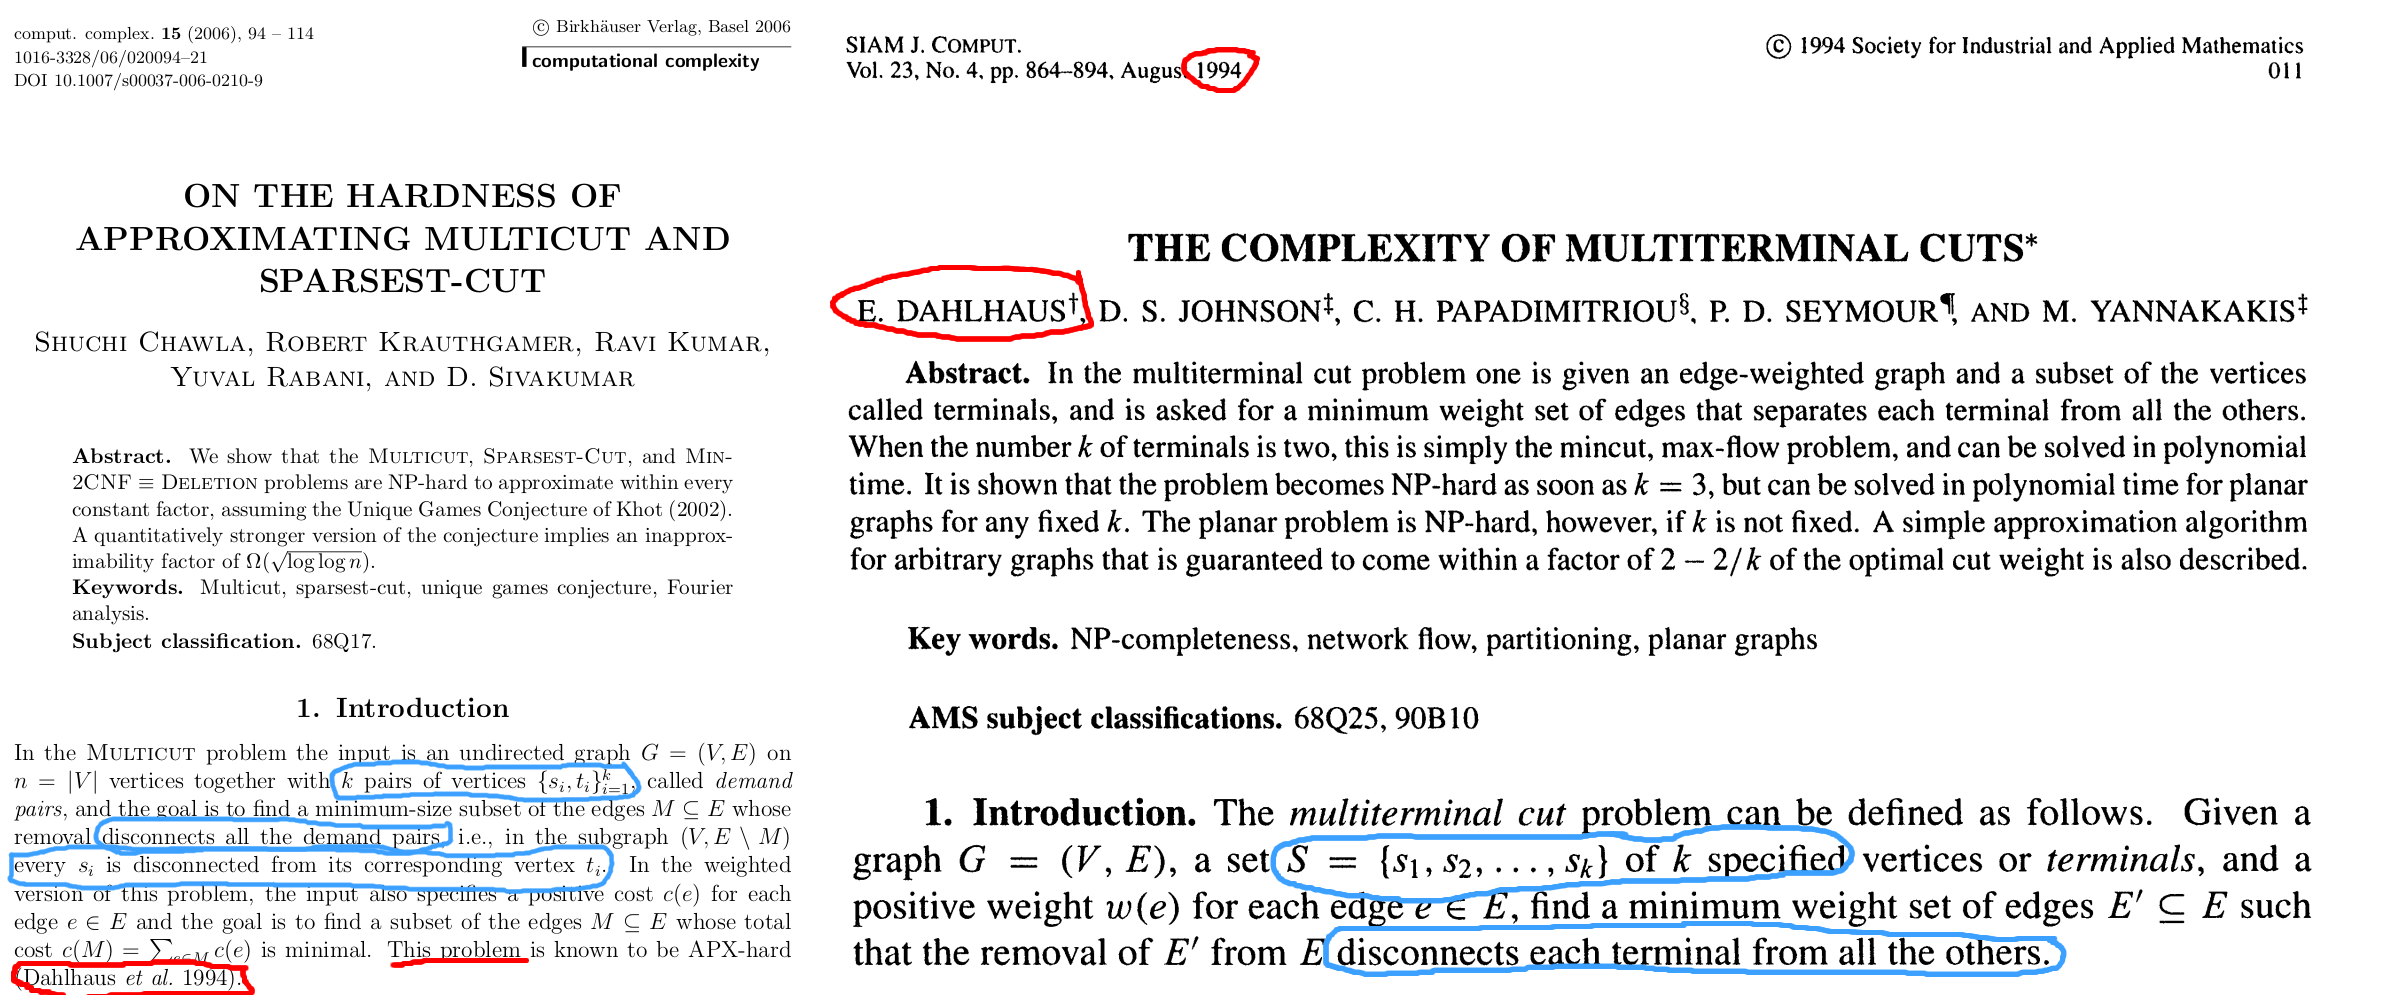
\includegraphics[width=0.9\linewidth]{assets/raw/multicut_vs_multiway.png}
   \caption{Confusing statement} \label{fig:cc_multiwhat}
\end{figure}


% \enquote{We prove that if the Unique Games Conjecture of Khot (2002) is true, then for every constant L > 0
% it is NP-hard to approximate Multicut within factor L. If a quantitatively stronger version of the
% conjecture is true, then Multicut is NP-hard to approximate within a factor of $\Omega(\sqrt{\log
% \log n})$.}

% It's probably limited because LP with a lot of constraints do not scale that well (someone claimed
% $O(n^{4.5})$)

% SDP Gaps and UGC Hardness for Multiway Cut, 0-Extension and Metric Labelling,
% On the Unique Games Conjecture: Subhash Khot
% under the UGC, one cannot get better than $O(\log n)$ approximation using LP or SDP relaxation.
